% Template file for an a0 landscape poster.
% Written by Graeme, 2001-03 based on Norman's original microlensing
% poster.
%
% See discussion and documentation at
% <http://www.astro.gla.ac.uk/users/norman/docs/posters/> 
%
% $Id: poster-template-landscape.tex,v 1.2 2002/12/03 11:25:46 norman Exp $


% Default mode is landscape, which is what we want, however dvips and
% a0poster do not quite do the right thing, so we end up with text in
% landscape style (wide and short) down a portrait page (narrow and
% long). Printing this onto the a0 printer chops the right hand edge.
% However, 'psnup' can save the day, reorienting the text so that the
% poster prints lengthways down an a0 portrait bounding box.
%
% 'psnup -w85cm -h119cm -f poster_from_dvips.ps poster_in_landscape.ps'

\documentclass[a0]{a0poster}
% You might find the 'draft' option to a0 poster useful if you have
% lots of graphics, because they can take some time to process and
% display. (\documentclass[a0,draft]{a0poster})
\input defs
\pagestyle{empty}
\setcounter{secnumdepth}{0}
\renewcommand{\familydefault}{\sfdefault}
\newcommand{\QED}{~~\rule[-1pt]{8pt}{8pt}}\def\qed{\QED}

\renewcommand{\reals}{{\mbox{\bf R}}}

% The textpos package is necessary to position textblocks at arbitary 
% places on the page.
\usepackage[absolute]{textpos}

\usepackage{fleqn,psfrag,wrapfig,tikz}

\usepackage[papersize={38in,28in}]{geometry}

% Graphics to include graphics. Times is nice on posters, but you
% might want to switch it off and go for CMR fonts.
\usepackage{graphics}


% we are running pdflatex, so convert .eps files to .pdf
%\usepackage[pdftex]{graphicx}
%\usepackage{epstopdf}

% These colours are tried and tested for titles and headers. Don't
% over use color!
\usepackage{color}
\definecolor{Red}{rgb}{0.9,0.0,0.1}

\definecolor{bluegray}{rgb}{0.15,0.20,0.40}
\definecolor{bluegraylight}{rgb}{0.35,0.40,0.60}
\definecolor{gray}{rgb}{0.3,0.3,0.3}
\definecolor{lightgray}{rgb}{0.7,0.7,0.7}
\definecolor{darkblue}{rgb}{0.2,0.2,1.0}
\definecolor{darkgreen}{rgb}{0.0,0.5,0.3}

\renewcommand{\labelitemi}{\textcolor{bluegray}\textbullet}
\renewcommand{\labelitemii}{\textcolor{bluegray}{--}}

\setlength{\labelsep}{0.5em}


% see documentation for a0poster class for the size options here
\let\Textsize\normalsize
%\def\Head#1{\noindent\hbox to \hsize{\hfil{\LARGE\color{bluegray} #1}}\bigskip}
\def\Head#1{\noindent{\LARGE\color{bluegray} #1}\bigskip}
\def\LHead#1{\noindent{\LARGE\color{bluegray} #1}\bigskip}
\def\Subhead#1{\noindent{\large\color{bluegray} #1}\bigskip}
\def\Title#1{\noindent{\VeryHuge\color{Red} #1}}


% Set up the grid
%
% Note that [40mm,40mm] is the margin round the edge of the page --
% it is _not_ the grid size. That is always defined as 
% PAGE_WIDTH/HGRID and PAGE_HEIGHT/VGRID. In this case we use
% 23 x 12. This gives us three columns of width 7 boxes, with a gap of
% width 1 in between them. 12 vertical boxes is a good number to work
% with.
%
% Note however that texblocks can be positioned fractionally as well,
% so really any convenient grid size can be used.
%
\TPGrid[40mm,40mm]{23}{12}      % 3 cols of width 7, plus 2 gaps width 1

\parindent=0pt
\parskip=0.2\baselineskip

% Our package definitions
\usepackage{optidef}
\usepackage{pspicture}
\usepackage{psfrag}
\usepackage{mathrsfs}
\usepackage{graphicx}
\usepackage{amsmath}
\usepackage{amsfonts}
\usepackage[small,bf]{caption}
\usepackage[usenames,dvipsnames]{pstricks}
\usepackage{epsfig}
%\usepackage{pst-grad} % For gradients
%\usepackage{pst-plot} % For axes
%\usepackage[space]{grffile} % For spaces in paths
%\usepackage{etoolbox} % For spaces in paths
\makeatletter % For spaces in paths
\patchcmd\Gread@eps{\@inputcheck#1 }{\@inputcheck"#1"\relax}{}{}
\makeatother

\newcommand{\linop}{\mathscr{L}}
\newcommand{\idop}{\mathbb{I}}
\newcommand{\ip}[1]{\left\langle{#1}\right\rangle}
\newcommand{\haml}{\mathcal{H}}

\begin{document}

% Understanding textblocks is the key to being able to do a poster in
% LaTeX. In
%
%    \begin{textblock}{wid}(x,y)
%    ...
%    \end{textblock}
%
% the first argument gives the block width in units of the grid
% cells specified above in \TPGrid; the second gives the (x,y)
% position on the grid, with the y axis pointing down.

% You will have to do a lot of previewing to get everything in the 
% right place.

% This gives good title positioning for a portrait poster.
% Watch out for hyphenation in titles - LaTeX will do it
% but it looks awful.
\begin{textblock}{23}(0,0)
\Title{Fast Eigenvalue Optimization for Spectral-Element PDEs}
\end{textblock}

\begin{textblock}{23}(0,0.6)
{
\LARGE
Guillermo Angeris and John Sholar
}

{
\Large
\color{bluegray}
\emph{EE364b: Convex Optimization II Class Project}
}
\end{textblock}


% Uni logo in the top right corner. A&A in the bottom left. Gives a
% good visual balance, but you may want to change this depending upon
% the graphics that are in your poster.
%\begin{textblock}{2}(0,10)
%Your logo here
%%\includegraphics{/usr/local/share/images/AandA.epsf}
%\end{textblock}

%\begin{textblock}{2}(21.2,0)
%Another logo here
%%\resizebox{2\TPHorizModule}{!}{\includegraphics{/usr/local/share/images/GUVIu/GUVIu.eps}}
%\end{textblock}


\begin{textblock}{7.0}(0,1.5)

\hrule\medskip
\Head{Introduction}\\
Eigenvalue optimization is a common task in many control problems, inverse design, and, recently, in inference problems on continuous spaces. In this project, we'll attempt to write a fast solver for eigenvalue problems arising from spectral element discretizations of eigenvalue partial differential equations (PDEs).

\hrule\medskip
\Head{Spectral Element Methods and Laplacian Construction} \\
A \textit{spectral element method} (SEM)\footnote{Note that this is a class of methods, each generated by different polynomials or quadrature rules.[SOURCE]} is a finite-element method for solving PDEs which makes use of high-degree polynomials to approximate functions on a compact domain. The idea is to construct a quadrature rule such that all polynomials of lesser degree have exact integrals when sampled at a particular set of points and use these polynomials as a basis to approximate functions.

In general, these SEM-discretized problems---while sparse---are usually slow to solve in modern optimization packages for even a modest number of points in the discretization domain as they lack the tridiagonal structure that many PDE problems have (e.g., when discretizing by assuming $h^2f''(x) \approx f(x+h) - 2f(x) + f(x-h)$ for fixed $h>0$). In particular, the matrix generated by the spectral elements method is essentially a block-diagonal matrix with small blocks, each of which overlap with the previous block by exactly one element (see Figure~\ref{fig:overlap}), so no completely trivial decomposition can be applied.\footnote{Further, it's important to note that this matrix sparsity pattern is a special case of chordal sparsity [SOURCE], which, while fast to solve in general, does not take advantage of the further structure which is obvious from this problem.}

\begin{figure} \label{fig:overlap}
\begin{center}
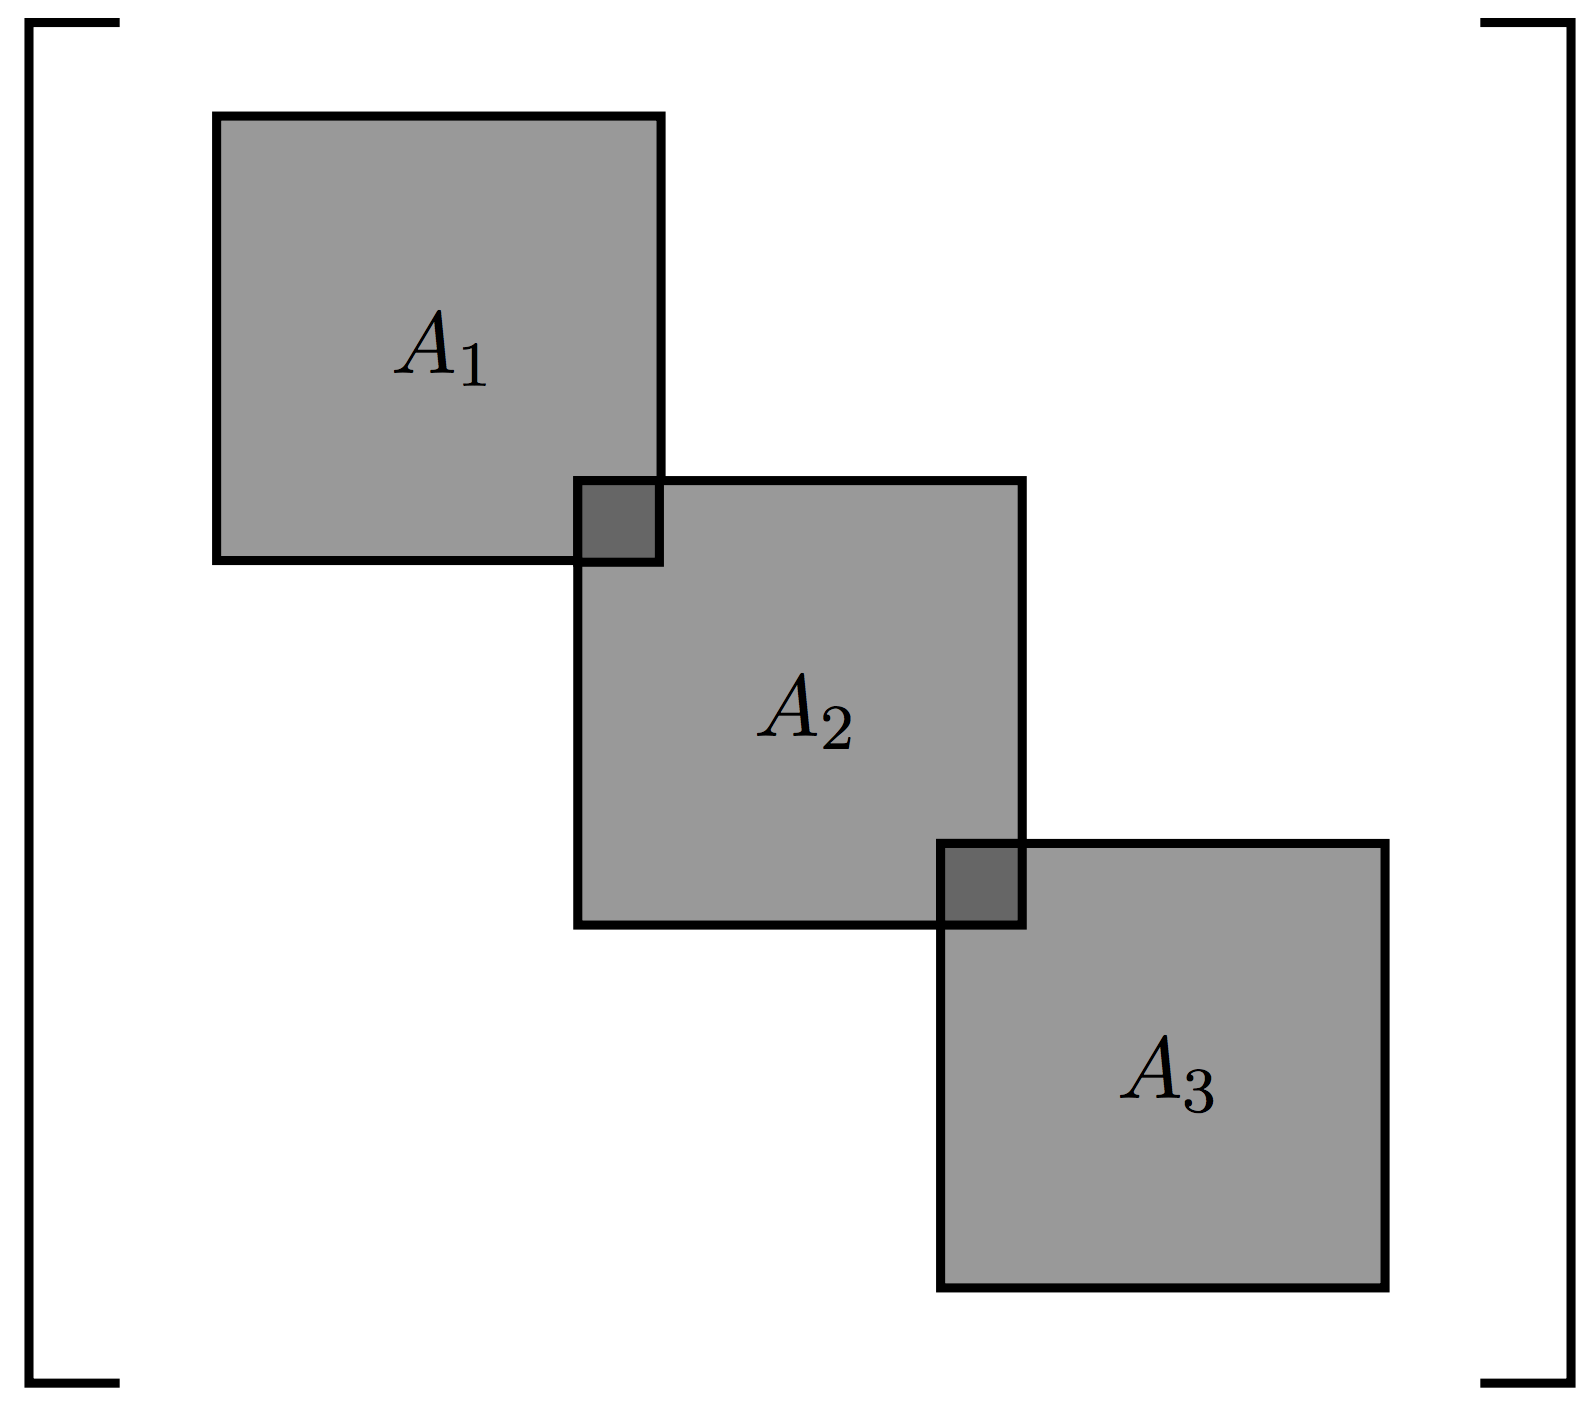
\includegraphics[width=\textwidth]{figures/overlap.png}
\caption{A simple example of the overlapping diagonal elements with three blocks. The darker box indicates a single overlapping element, e.g., $(A_1)_{nn} = (A_2)_{11}$ if $A_1 \in \reals^{n\times n}$.}
\end{center}
\end{figure}
Our project will take advantage of the structure of these approximately-block-diagonal matrices for fast solutions of eigenvalue problems.

\end{textblock}

\begin{textblock}{7.0}(8,1.5)

\medskip
\hrule\medskip
\Head{Approaches}\\
Let $\linop: \reals^n \to \symm^m$ be affine and have the approximately-block-diagonal structure described in figure \ref{fig:overlap} and let $x \in \reals^n$, then the problem of interest can be written as the dual of a standard-form SDP,
\begin{mini}
{x, t}{-b^Tx + t}{}{}
\addConstraint{\linop(x)}{\lek tI}
\addConstraint{Cx}{=d}
\addConstraint{x}{\gek 0}.
\end{mini}
The first inequality is with respect to the semidefinite cone, while the latter is with respect to the positive orthant

This general optimization problem can be solved in several ways. We will attempt to explore three possibilities: interior point methods for solving these large-scale SDPs, first-order cone-splitting methods, and a consensus approach for solving these problems. 

\medskip
\hrule\medskip
\Head{Interior Point Methods}\\
For interior point methods, rewriting the problem using a barrier method is straightforward
\begin{mini*}
{x, t}{-b^Tx + t - \mu\log \det (tI - \linop(x))}{}{}
\addConstraint{Cx}{=d}
\addConstraint{x}{\gek 0}.
\end{mini*}

\medskip
\hrule\medskip
\Head{First-Order Cone-Splitting Methods}\\
In the second case, define $E_i \in \reals^{d\times m}$ to be the `selection matrix' given by
\[
E_i = \underbrace{\begin{bmatrix}
\underbrace{\begin{matrix}0_{d \times (d-1)} & \dots & 0_{d \times (d-1)}\end{matrix}}_{i-1} & I_d & 0_{d \times (d-1)} & \dots & 0_{d \times (d-1)}
\end{bmatrix}}_{b}.
\]
where $b$ is the number of sub-blocks of $\linop$ and $d$ is their dimension.

This allows us to rewrite~(\ref{eq:optim}) above to
\begin{mini*}
{x, t}{-b^Tx + t}{}{}
\addConstraint{\linop(x) - tI}{=\sum_i E_i Z_i E_i^T} 
\addConstraint{Cx}{=d}
\addConstraint{x}{\gek 0}
\addConstraint{Z_i}{\gek 0,}{~ i\in\{1, 2, \dots, b\}},
\end{mini*}
where projecting the much smaller $Z_i$ matrices (if $d \ll m$, as is the case with the motivating example described in section ) into the PSD cone is much faster than projecting $\linop(x) - tI$.

\end{textblock}

\begin{textblock}{7.0}(8,1.5)

\end{textblock}

\end{document}
